\section{Дифференциальная эволюция.}

Предложена в 1997 году и предназначенная для решения задач, заданных на  $R^n$.

\begin{itemize}
      \item Мутация в ней – это линейная комбинация нескольких решений
      \item Скрещивание в ней, как правило, однородное
   \end{itemize}

Проходим по всем особям, выбираем три особи a,b,с отличные от текущей особи и получаем особь  d  за счет линейной комбинации особей a,b,c.  Далее получаем решение е как кроссовер текущей особи и особи d. Сохраняем либо текущую особь, либо особь е. Повторяем весь процесс до тех пор пока не найдем достаточно хорошее решение или есть время.

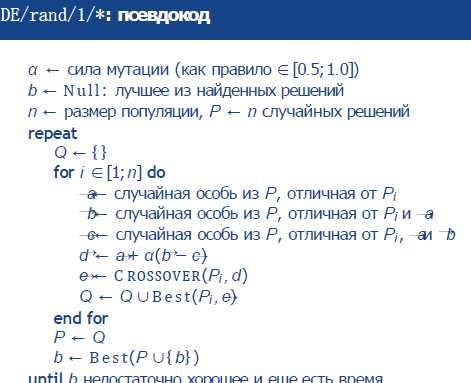
\includegraphics[width=300]{images/15bilet.png}  